 \documentclass [12pt]{article} 

\usepackage {amsmath}
\usepackage {amsthm}
\usepackage {amssymb}
\usepackage {graphicx} 
\usepackage {float}
\usepackage {multirow}
\usepackage {xcolor}
\usepackage [ruled,vlined,commentsnumbered,titlenotnumbered]{algorithm2e} \usepackage {array} 
\usepackage {booktabs} 
\usepackage {url} 
\usepackage {parskip} 
\usepackage [margin=1in]{geometry} 
\usepackage [T1]{fontenc} 
\usepackage {cmbright} 
\usepackage [many]{tcolorbox} 
\usepackage [colorlinks = true,
            linkcolor = blue,
            urlcolor  = blue,
            citecolor = blue,
            anchorcolor = blue]{hyperref} 
\usepackage {enumitem} 
\usepackage {xparse} 
\usepackage {verbatim}
\usepackage{algpseudocode}
\usepackage{listings}
\usepackage{xcolor}
\lstset { %
    language=C++,
    backgroundcolor=\color{black!5}, % set backgroundcolor
    basicstyle=\footnotesize,% basic font setting
}
\newtheorem{theorem}{Theorem}
\newtheorem{remark}{Remark}
\newtheorem{lemma}[theorem]{Lemma}
\theoremstyle{definition}
\newtheorem{definition}{Definition}[section]
\newtheorem{claim}{Claim}
\newtheorem{proposition}{Proposition}






\DeclareTColorBox {Solution}{}{breakable, title={Solution}} \DeclareTColorBox {Solution*}{}{breakable, title={Solution (provided)}} \DeclareTColorBox {Instruction}{}{boxrule=0pt, boxsep=0pt, left=0.5em, right=0.5em, top=0.5em, bottom=0.5em, arc=0pt, toprule=1pt, bottomrule=1pt} \DeclareDocumentCommand {\Expecting }{+m}{\textbf {[We are expecting:} #1\textbf {]}} \DeclareDocumentCommand {\Points }{m}{\textbf {(#1 pt.)}} 

\begin {document} 

\vspace {1em} 
\begin {Instruction} 
Adapted From Virginia Williams'lecture notes.
\end {Instruction}  

{\LARGE \textbf {COMP 285 (NC A\&T, Spr `22)}\hfill \textbf {Lecture 31} } 

\begin{centering}
\section*{Minimum Spanning Trees}
\end{centering}

\section{Introduction}

Today we will continue our discussion of greedy algorithms, specifically in the context of computing minimum spanning trees. There are many useful applications for finding a minimum spanning tree of a graph from efficient network design to graph clustering analysis and
much more. We will also show that we can compute a minimum spanning tree of a graph in
polynomial time using some intuitive greedy algorithms.
 
The minimum spanning tree problem is formulated informally as follows: we are provided an undirected graph $G = (V, E)$ with weights $w(e) \in R$ for $e \in E$ and we want to compute a subgraph of $G$ that is a tree which connects all vertices in $V$ (a spanning tree) and has minimum total edge weight defined as $w(T) = \sum_{e\in T} w(e)$.

Below is an example of an MST of a graph. In the example, the edges forming the MST are colored blue while edges that are not part of the MST are colored black:


\begin{figure}[h!]
\centering
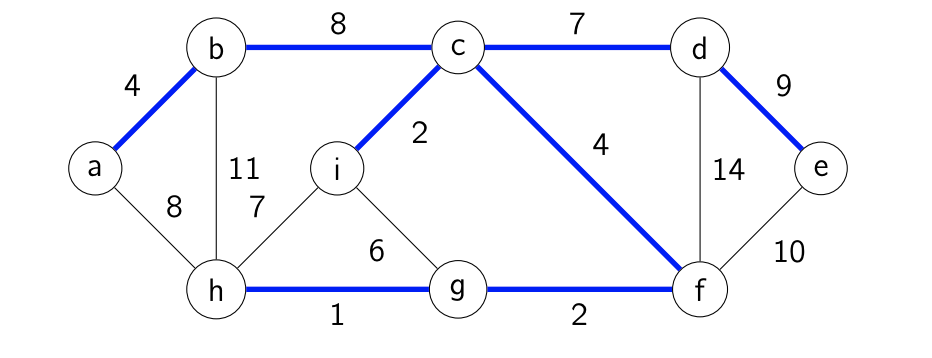
\includegraphics[scale=0.5]{mst_example.png}
\end{figure}

\section{ A Template for Minimum Spanning Tree Algorithms}
Let;s start by introducing a basic algorithm template which will guide our discussion towards the actual algorithms for computing MSTs. These algorithms will in general follow the steps described in the template below: 

We will show that the template results in a valid MST by maintaining the invariant that there exists at least one MST which contains all the edges in $A$. An edge is considered safe to add to A as long as it maintains this invariant. We will see that this definition of a safe edge can informally be defined as the edge with minimum weight which would not form a cycle if included in $A$. The next section will introduce new terminology to define this formally.

\begin{algorithm}
\caption{Template for Minimum Spanning Tree Algorithms}
\label{alg:mst_template}
\begin{algorithmic}
\State $A \gets \emptyset$
\State \While{$A$ is not a spanning tree} {
    \State find edge $(u,v)$ that is 'safe' for $A$
    \State $A \gets A \cup \{(u,v)\}$
}
\State \Return $A$
\end{algorithmic}
\end{algorithm}

\section{Cuts and Light Edges}
 
We will introduce the notion of graph cuts to formally discuss which edges can be considered safe to add to the MST edge set. Let a cut $(S, V \setminus S)$ of a graph $G = (V, E)$ be a partition of $V$ into two disjoint sets $S$ and $V \setminus S$. From this, we can say that an edge $$(u, v )$$ crosses the cut $(S, V \setminus S)$ if the edge has one endpoint in $S$ and the other in $V \setminus S$. We can also say that a cut respects a subset $A$ of edges if no edges in $A$ cross the cut. An edge is considered a light edge crossing a cut if its weight is the minimum of any edge crossing the cut.

\begin{figure}[h!]
\centering
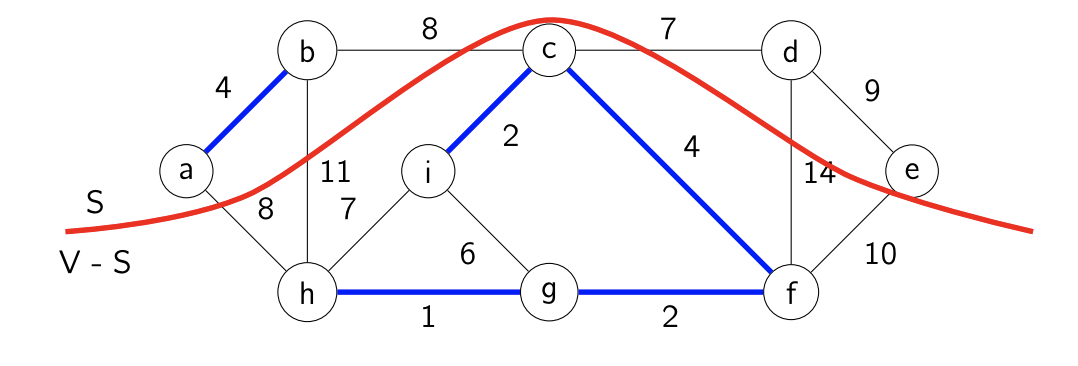
\includegraphics[scale=0.5]{mst_cuts.png}
\label{}
\label{fig:mst_cuts}
\end{figure}

In the example above (Figure \ref{fig:mst_cuts}), let $(S, V \setminus S)$ be a cut of the graph where $S$ contains the set of nodes above the red curve and $V \setminus S$ contains the set of nodes below it, and the set $A$ be the set of edges colored blue. The edges which cross the cut are exactly the following: $(a, h), (b, h), (b, c), (c, d), (d, f ), (e, f )$ and the only light edge which crosses $(S, V \setminus S)$ is $(c, d)$. Since none of these edges are contained in the set $A$, the cut respects the set $A$. Note that if we were to add any of the edges previously mentioned to $A$, then the cut would
no longer respect $A$.

Given the definitions above, let $G = (V, E)$ be a connected and undirected graph with edge weights $w(e)$, $A$ be a subset of $E$ such that some MST of $G$ contains $A$, ($S, V \setminus S)$ be a cut that respects $A$, and $(u, v )$ be a light edge crossing $(S, V \setminus S)$.

\begin{theorem}
There exists an MST that contains $A \cup \{(u,v)\}$.
\label{thm:lemma}
\end{theorem}

\begin{proof} 
Let $T$ be an MST containing $A$. As previously mentioned, $(u, v )$ is a light edge which crosses the cut $(S, V \setminus S)$. Since $T$ is already a spanning tree, note that adding any other edge of the graph to it will lead to a cycle, so in particular adding $(u, v )$ to $T$ produces a cycle. Consider a path $p$ from $u$ to $v$ in $T$. There will necessarily be at least one edge $(x, y )$ of $p$ which crosses the cut $(S, V \setminus S)$ where $(x, y ) \notin A$ because the cut respects $A$. Since $(u, v )$ is a light edge, w$(u, v ) \leq w(x, y )$. Deleting $(x, y )$ from $T$ and adding $(u, v )$ yields a new MST $T'$ . The only difference between $T$ and $T'$ are the edges $(x, y )$ and $(u, v )$ so $w(T') \leq w(T)$. $T'$ is an MST which contains $A \cup \{(u, v )\}$.
\end{proof}

\begin{figure}[h!]
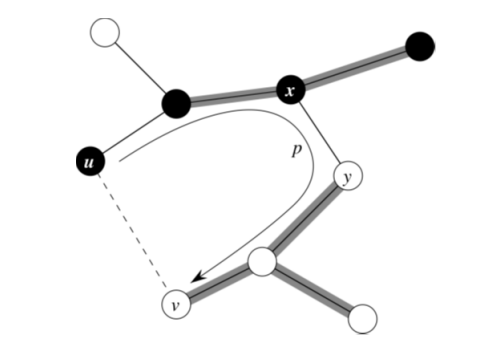
\includegraphics[scale=0.5]{mst_proof.png}
\end{figure}
 
Note that in the proof, if $w(T') \neq w(T)$, then we have that our initial assumption of $T$ being an MST is false since we have found a spanning tree with smaller total edge weight. Because of the theorem, we can add some additional points about the MST algorithm template. 

\begin{itemize}
    \item The MST algorithm maintains a subset $A$ of edges with no cycles. That is, the graph represented by $G_A = (V, A)$ is a forest (a set of distinct unconnected trees). 
    \item Any safe edge $(u, v )$ connects two distinct connected components of $G_A$. 
    \item For some connected component $C = (V_C, E_C)$ in $G_A$, the safe edge $(u, v )$ is a light edge crossing $(V_C, V \setminus V_C)$.
\end{itemize}

\section{Prim's Algorithm}
 
At a high level, the set $A$ maintained by Prim's algorithm is a single tree. The algorithm starts with an arbitrary root $r$ and in each step, a light edge leading out of $A$ and connecting to a node that has not yet been connected to $A$ is selected and added to $A$. Once $A$ connects every node in the graph, it is returned as an MST of the graph. 

Prim's algorithm is similar to Dijkstra's algorithm in that estimates of the distance to each
node are maintained and updated as the algorithm progresses. $Q$ is a priority queue maintaining distances of vertices not in the tree so far, $key(v )$ is the minimum weight of edge connecting $v$ to some vertex in the tree, and $p(v )$ is the parent of $v$ in the tree.

\textbf{Correctness} Much of the correctness of Prim's algorithm follows from Theorem \ref{thm:lemma}. Notice that at the beginning of every loop iteration, $A = \{ (p(v ), v ) : v \in (V \setminus  \{r\} \setminus  Q)\}$ meaning that the vertices already placed in the partial MST are those in $V \setminus Q$. For all vertices $v \in Q$, if $p(v ) \neq \texttt{NIL}$, then $key(v )$ is the minimum weight of an edge connecting v to the partial MST. This can be thought of in terms of graph cuts with partitions $(Q, V \setminus Q)$ and the vertices in $Q$ with non-\texttt{NIL} parents as being the tail of edges crossing this cut. Since in $Q$,
only the vertices with non-\texttt{NIL} parents have key $\neq \infty$ (except for $r$ in the first iteration), this means that only the edges which cross the cut are considered at each iteration and the one with minimum weight is added to $A$. This is exactly what the MST template algorithm does (we add a safe edge) and as such, the correctness of the algorithm follows.

\begin{algorithm}
\caption{Prim($G$)}
\label{alg:prims_algorithm}
\begin{algorithmic}
\State key($v) \gets \infty, \forall v \in V$
\State key($r) \gets 0$
\State $Q \gets (\text{key}(v), v), \forall v \in V$
\State $p(v) \gets \texttt{NIL}, \forall v \ in V$
\State $A \gets \emptyset$
\State \While{$Q$ is not empty} {
    \State $u \gets $ ExtractMin($Q$)
    \State \If{$u \neq r$} {
        \State $A = A \cup \{(p(u),u) \}$
    }
    \State \For{each neighbor $v$ of $u$} {
        \State \If {$v \in Q$ and $w(u,v) < \text{key}(v)$} {
            \State key($v) = w(u,v)$
            \State DecreaseKey(key($v$), $v$)
            \State $p(v) = u$
        }
    }
}
\State \Return $A$
\end{algorithmic}
\end{algorithm}

\textbf{Running time} Prim's Algorithm can be implemented as a direct modification of Dijkstra's Algorithm and can achieve a similar running time, but its exact bound depends on the implementation of the priority queue.

If a red-black tree or a binary heap is used:
\begin{itemize}
    \item ExtractMin: $O(log n)$
    \item DecreaseKey: $O(log n)$
    \item Total: $O(n log n + m log n) = O(m log n)$
\end{itemize}

If a Fibonacci heap is used:
\begin{itemize}
    \item ExtractMin: $O(log n)$
    \item DecreaseKey: $O(1)$ amortized
    \item Total: $O(n log n + m)$
\end{itemize}

\textbf{Example} In this example, we will run through the steps fo Prim's algorithms in order to find an MST for the graph in Figure \ref{fig:prims_1}:

\begin{figure}[h!]
\centering
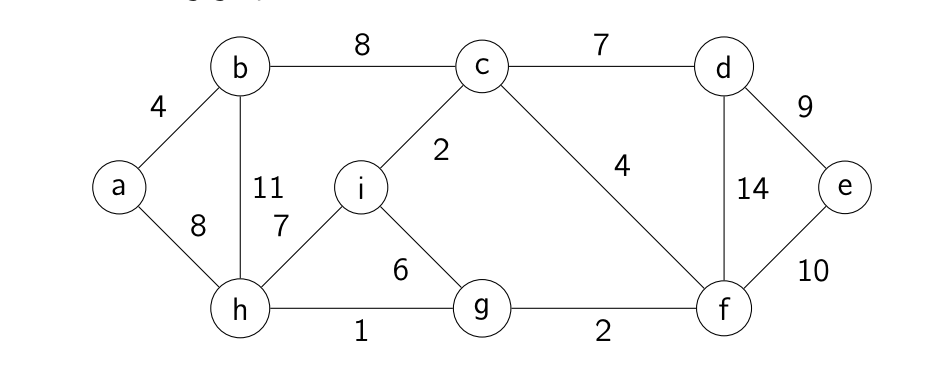
\includegraphics[scale=0.8]{prims_1.png}
\caption{}
\label{fig:prims_1}
\end{figure}

Suppose we select node a to be the source node, $r$. We then extract node $a$ from $Q$ and set key$(b) = 4$ , $p(b) = a$, key$(h) = 8$, and $p(h) = a$ as shown in Figure \ref{fig:prims_2}.

\begin{figure}[h!]
\centering
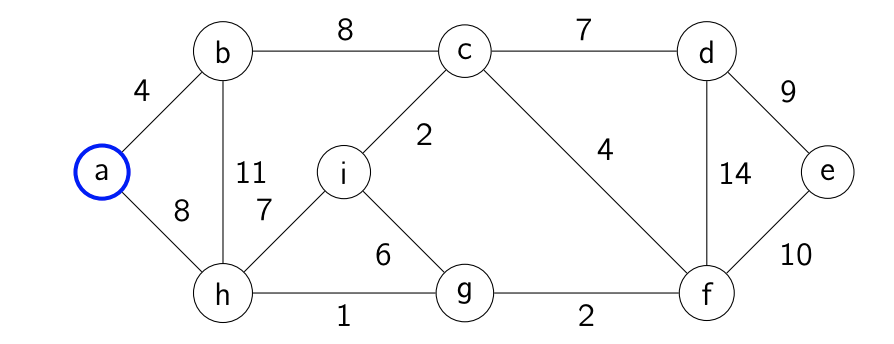
\includegraphics[scale=0.8]{prims_2.png}
\caption{}
\label{fig:prims_2}
\end{figure}

Since key$(b)$ is now the smallest value in the priority queue, we visit node $b$. Because $p(b) = a$ we add edge $(a, b)$ to the set $A$. We then update the keys and parent fields of nodes that have edges connecting to $b$. Thus we set key$(c) = 8$ and $p(c) = b$ as shown in Figure \ref{fig:prims_3}.

\begin{figure}[h!]
\centering
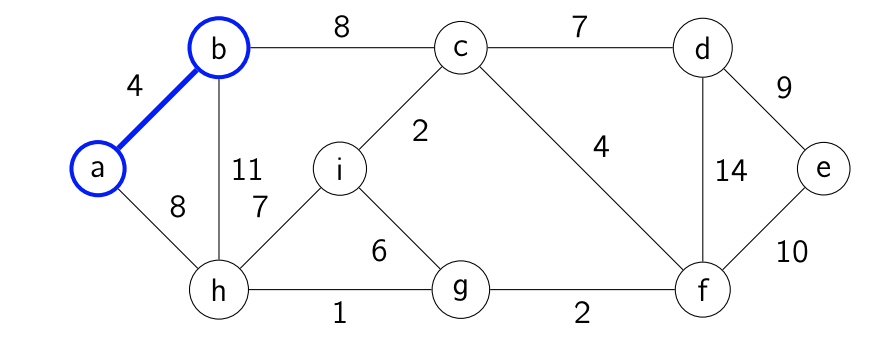
\includegraphics[scale=0.8]{prims_3.png}
\caption{}
\label{fig:prims_3}
\end{figure}

The next smallest in the priority queue is a tie between key$(c)$ and key$(h)$. The algorithm can pick either one - the results may be different, but both will be an MST. Let's say the algorithm arbitrarily picks $c$. We add edge $(b, c)$ to $A$ and perform the following updates: key$(d) = 7$, $p(d) = c$, key$(f ) = 4$, $p(f ) = c$, key($i) = 2$, and $p(i) = c$ as shown in Figure \ref{fig:prims_4}.

\begin{figure}[h!]
\centering
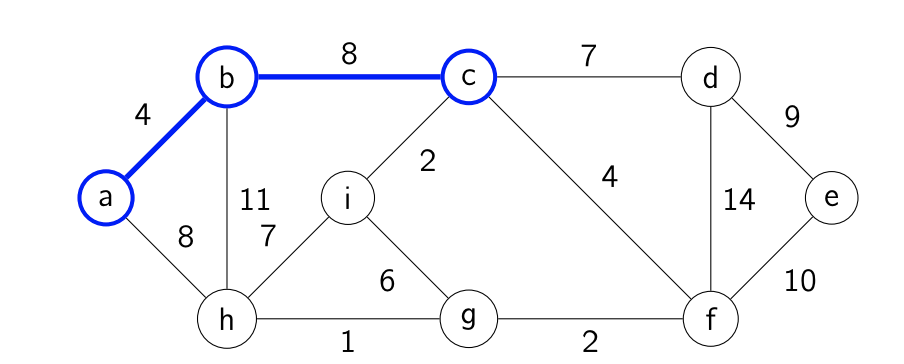
\includegraphics[scale=0.8]{prims_4.png}
\caption{}
\label{fig:prims_4}
\end{figure}

key$(i)$ is the smallest so we visit node $i$. Update the following: key$(g) = 6$, $p(g) = i$, key$(h)= 7$, and $p(h) = i$ as shown in Figure \ref{fig:prims_5}.

\begin{figure}[h!]
\centering
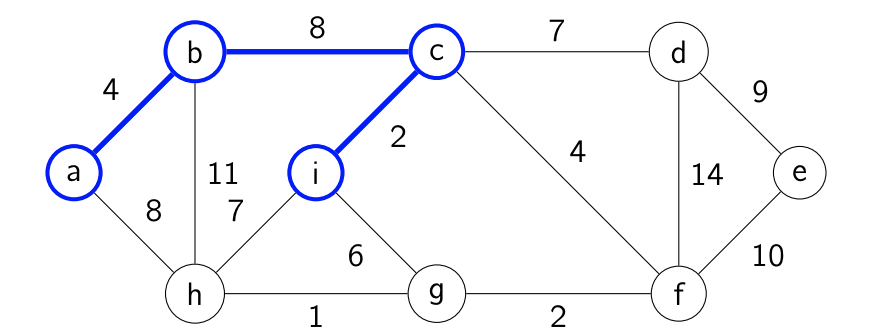
\includegraphics[scale=0.8]{prims_5.png}
\caption{}
\label{fig:prims_5}
\end{figure}

key$(f )$ is the smallest so we visit node $f$. Update the following: key$(g) = 2$, $p(g) = f$ , key$(e) = 10$, and $p(e) = f $ as shown in Figure \ref{fig:prims_6}.

\begin{figure}[h!]
\centering
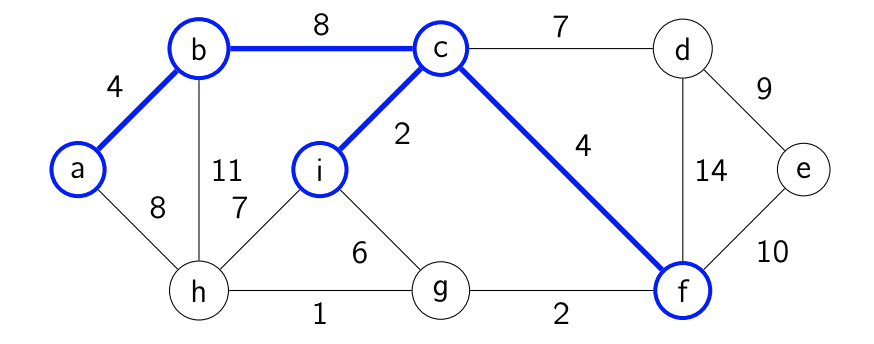
\includegraphics[scale=0.8]{prims_6.png}
\caption{}
\label{fig:prims_6}
\end{figure}

key$(g)$ is the smallest so we visit node $g$. Update the following: key$(h) = 1$ and $p(h) = g$ as shown in Figure \ref{fig:prims_7}.

\begin{figure}[h!]
\centering
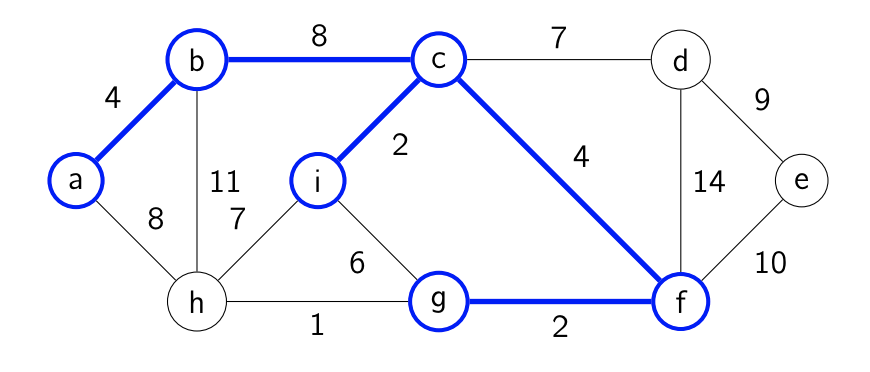
\includegraphics[scale=0.8]{prims_7.png}
\caption{}
\label{fig:prims_7}
\end{figure}

key$(h)$ is the smallest so we visit node $h$. There are no updates at this step as shown in Figure \ref{fig:prims_8}.

\begin{figure}[h!]
\centering
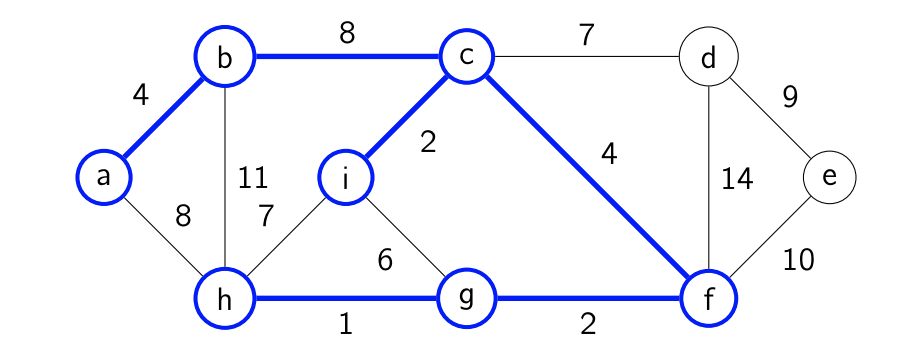
\includegraphics[scale=0.8]{prims_8.png}
\caption{}
\label{fig:prims_8}
\end{figure}

key$(d)$ is the smallest so we visit node $d$. Update the following: key$(e) = 9$ and $p(e) = d$ as shown in Figure \ref{fig:prims_9}.

\begin{figure}[h!]
\centering
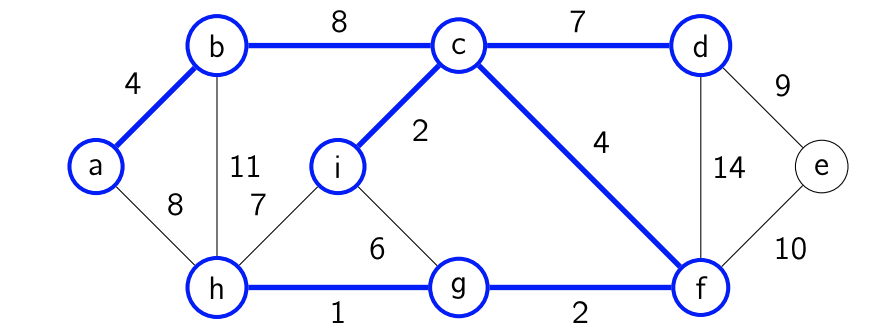
\includegraphics[scale=0.8]{prims_9.png}
\caption{}
\label{fig:prims_9}
\end{figure}

Finally, key$(e)$ is the smallest so we visit node $e$. There are no updates at this step and the algorithm will detect that $Q$ is empty at the next iteration and return as shown in Figure \ref{fig:prims_10}.

\begin{figure}[h!]
\centering
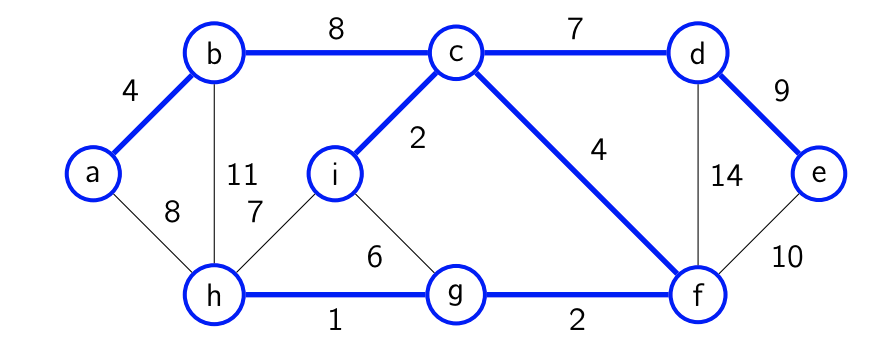
\includegraphics[scale=0.8]{prims_10.png}
\caption{}
\label{fig:prims_10}
\end{figure}


\section{Kruskal's Algorithm} 

At a high level, the set A maintained by Kruskal's algorithm is a set of disjoint trees. During update step $i$, if the ith smallest edge connects different trees, merge the two trees connected by this edge. The algorithm progresses until eventually only one tree remains at which point the set A represents an MST of the graph.

Kruskal's algorithm utilizes the union-find (aka disjoint set) data structure in order to handle the merging of the disjoint trees maintained by the algorithm. The union-find data structure supports disjoint sets with the following operations:

\begin{itemize}
\item \textbf{makeset}$(u)$: creates a new set containing $u$ provided that $u$ is not in any other set
\item \textbf{find}$(u)$: returns the name of the set containing $u$
\item \textbf{union}$(u, v )$: merge the set containing $u$ and the set containing $v$ into one set
\end{itemize}

The algorithm itself can be structured as follows:

\begin{algorithm}
\caption{Kruskal($G$)}
\label{alg:kruskal_algorithm}
\begin{algorithmic}
\State $A \gets \emptyset$
\State $E' \gets$ sort edges by weight in non-decreasing order
\State \For{ $v \in V$} {
    \State makeset(v)
}
\State \For{ $(u,v) \in E'$} {
    \If{find($u) \neq $ find(v)} {
        \State $A \gets A \cup \{(u,v)\}$
        \State union(u,v)
    }
}
\State \Return $A$
\end{algorithmic}
\end{algorithm}

\textbf{Correctness} The correctness follows from Theorem \ref{thm:lemma}.


\textbf{Running time} 

The runtime of Kruskal's algorithm depends on two factors: the time to sort the edges by weight and the runtime of the union-find data structure operations. While $\Omega(m \log n)$ time is required for sorting the edges if we use comparison-based sorting, in many cases, we may be able to sort the edges in linear time. (Recall, that RadixSort can be used to sort the edges in $O(m)$ time if the weights are given by integers bounded by a polynomial in $m$.) In this case, the runtime is bounded by the runtime of the union-find operations and is given by $O(nT(\text{makeset}) + mT(\text{find}) +nT(\text{union}))$. The best known data structure supporting the union-find operations runs in amortized time $O(\alpha(n))$ where $\alpha(n)$ is the inverse Ackermann function. Interestingly, the value of the inverse Ackermann is tiny for all practical purposes: 
$$
\alpha(n) \leq 4, \forall n < \text{\# atoms in the universe}
$$

and thus for all practical purposes, the union-find operations run in constant time. Thus, in many settings, the runtime of Kruskal's algorithm is nearly linear in the number of edges. 

The actual definition of $\alpha(n)$ is $\alpha(n) = \min\{k \mid A(k) \geq n\}$, where $A(k)$ is the Ackermann function evaluated at $k$. $A(k)$ itself is defined using the more general Ackermann function as $A(k) = A_k(2)$. $A_k(x)$ is defined recursively: 

\begin{align*}
A_m(x) = 
    \begin{cases}
        x + 1 & m = 0 \\
        A_{m-1}(1) & m > 0, x = 0  \\
        A_{m-1}(A_m(x - 1)) & \text{ else }
    \end{cases}
\end{align*}

For example
\begin{itemize}
    \item $A_0(x) = 1 + x$, so $A_0(2) = 3$
    \item TO compute $A_1(x)$, we see:
    $$
    A_1(x) = A_0(A_1(x-1)) = A_0(A_0(A_1(x-2))) = \cdots = A_0(A_0(\cdots (A_0(A_1(0))))) = A_0(A_0(\cdots(A_0(2))))
    $$
    that is, we have ``iterated'' $A_0 x$ times. If we work it out, we get:
    $$
    A_1(x) = 2x
    $$
    Thus, $A_1(2) = 4$
    \item $A_2(x) = 2^x x$ ($A_1$ iterated $x$ times), so $A_2(2) = 8$ 
    \item $A_3(x) \geq 2^{2^{2^{2\cdots}}}$, a "tower" of $x$ 2s ($A_2$ iterated $x$ times); it turns out that $A_3(2) \geq 2^11$
    \item $A_4(x)$ is larger than the total number of atoms in the known universe, and also greater that the number of nanoseconds since the Big Bang. (Thus, $\alpha(n) \leq 4$ for all practice purposes)
\end{itemize}

\textbf{Example} In this example (Figure \ref{fig:kruskal0}) we will run through the steps of Kruskal's algorithm in order to find an MST for the following graph:


\begin{figure}[h!]
\centering
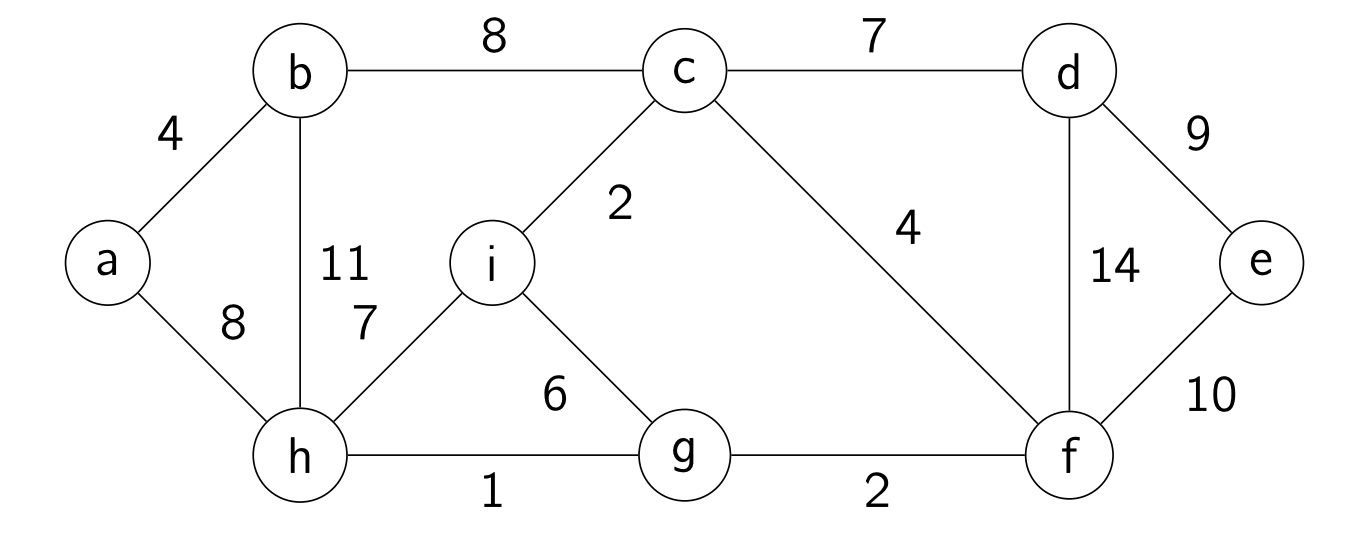
\includegraphics[scale=0.8]{kruskal0.png}
\caption{}
\label{fig:kruskal0}
\end{figure}
 
We begin by creating a new set for each node in the graph. We then begin iterating over the edges in non-decreasing order. The first edge we examine is $(g, h)$. This edge connects nodes $g$ and $h$ which are currently not part of the same set. We thus include this edge in $A$ and union the sets containing $g$ and $h$ as shown in Figure \ref{fig:kruskal1}.

\begin{figure}[h!]
\centering
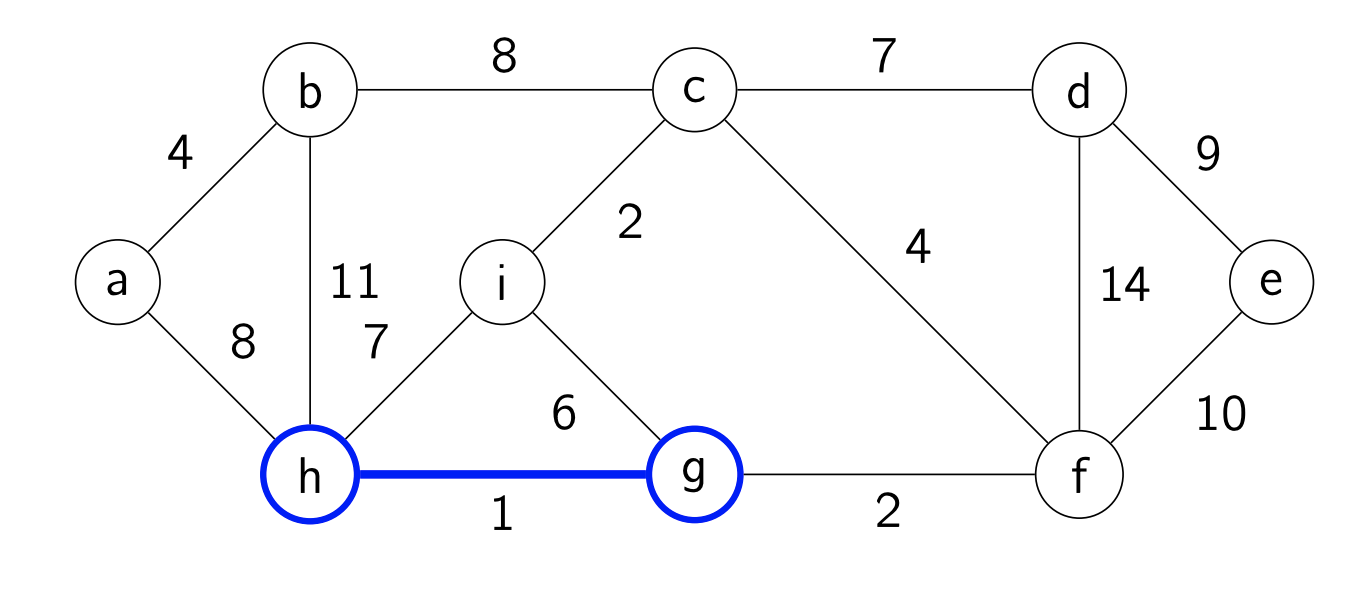
\includegraphics[scale=0.8]{kruskal1.png}
\caption{}
\label{fig:kruskal1}
\end{figure}

The next edge in the sorted order is a tie between edges $(c, i)$ and $(f , g)$. Picking either one will yield a correct result, so let’s say the algorithm picks $(c, i)$. Since $c$ and $i$ are not part of the same set we include this edge in $A$ and union the sets containing $c$ and $i$ as shown in Figure \ref{fig:kruskal2}.

\begin{figure}[h!]
\centering
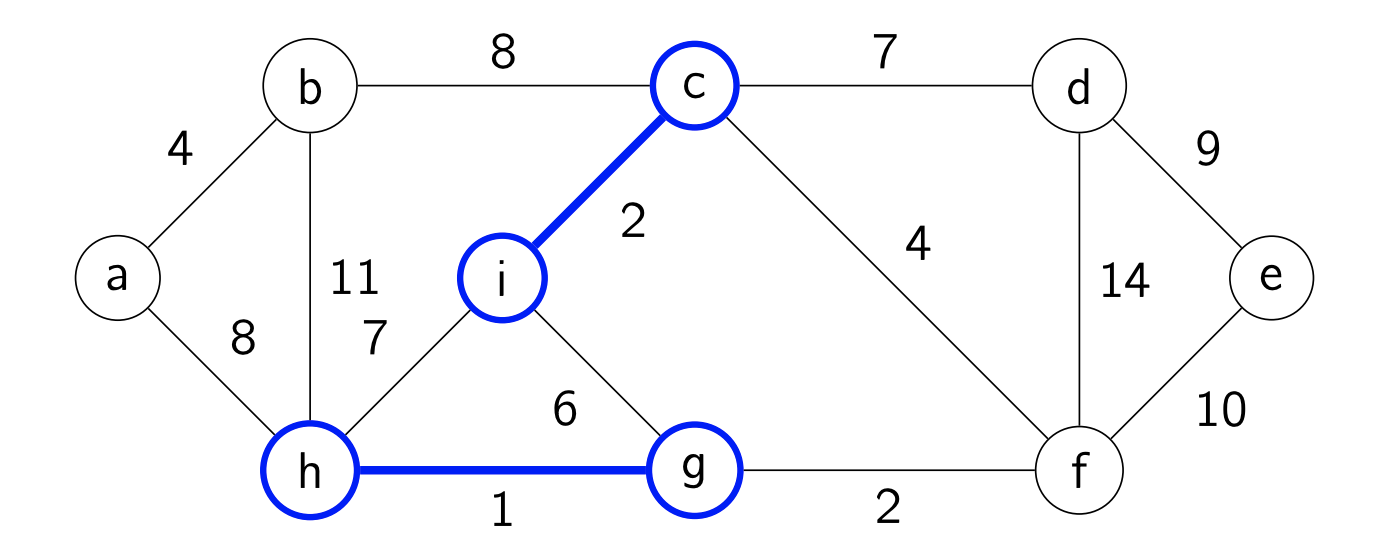
\includegraphics[scale=0.8]{kruskal2.png}
\caption{}
\label{fig:kruskal2}
\end{figure}



The next edge in the sorted order is $(f , g)$. We union the sets containing $f$ and $g$ and add edge $(f , g)$ to $ A$ as shown in Figure \ref{fig:kruskal3}.


\begin{figure}[h!]
\centering
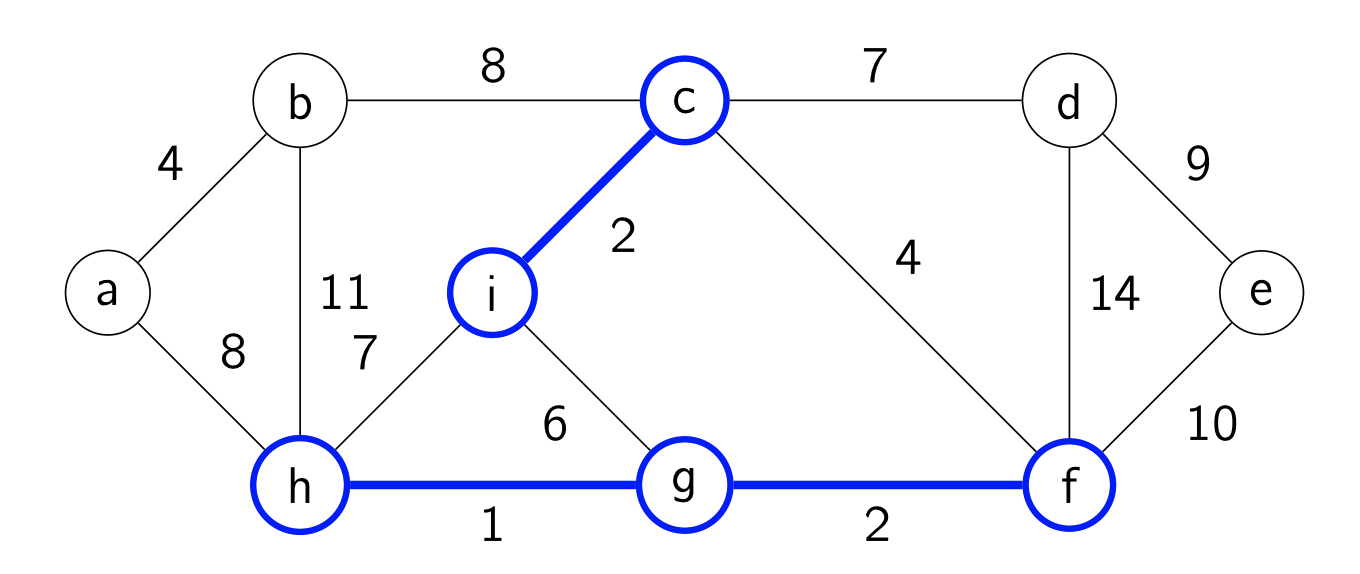
\includegraphics[scale=0.8]{kruskal3.png}
\caption{}
\label{fig:kruskal3}
\end{figure}

The next edge in the sorted order is a tie between edges $(a, b)$ and $(c, f )$. Let’s say the
algorithm picks $(a, b)$. We union the sets containing $a$ and $b$ and add edge $(a, b)$ to $A$ as shown in Figure \ref{fig:kruskal4}.

\begin{figure}[h!]
\centering
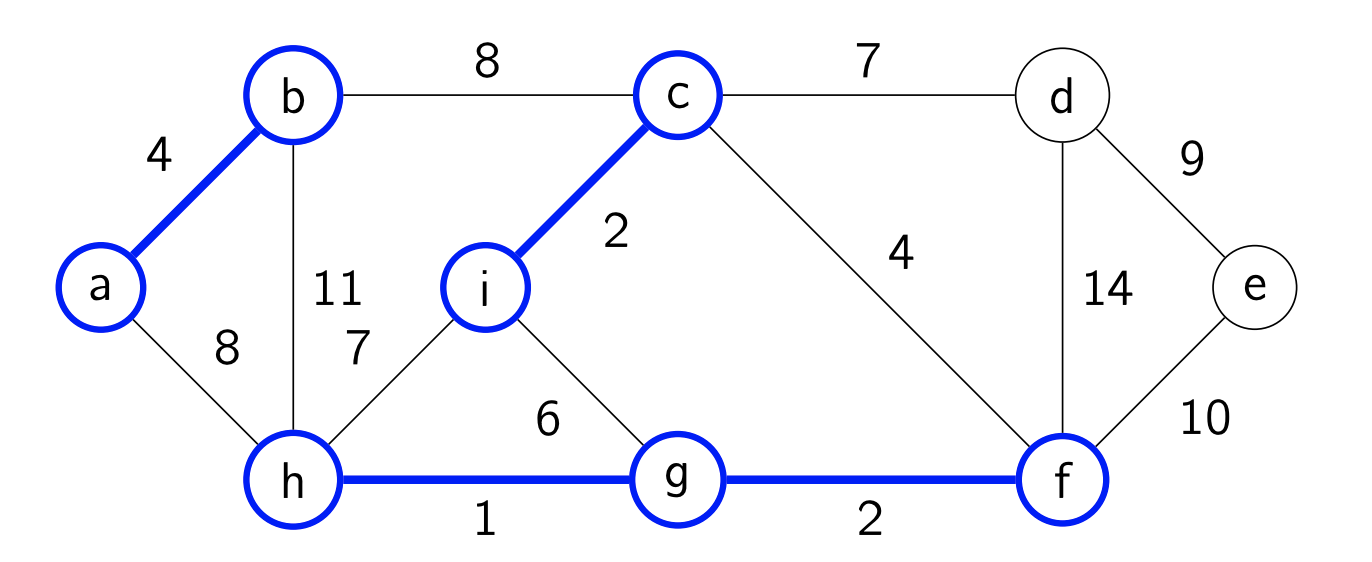
\includegraphics[scale=0.8]{kruskal4.png}
\caption{}
\label{fig:kruskal4}
\end{figure}


The next edge in the sorted order is $(c, f )$. We union the sets containing $c$ and $f$ and add edge $(c, f )$ to $A$ as shown in Figure \ref{fig:kruskal5}.

\begin{figure}[h!]
\centering
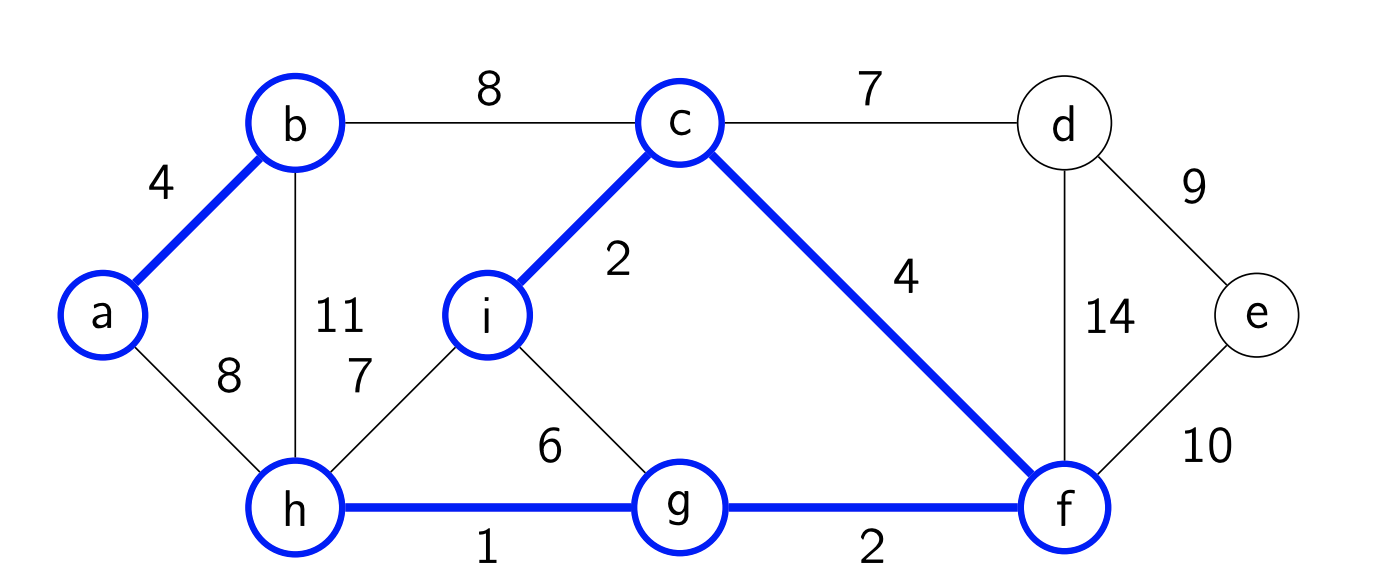
\includegraphics[scale=0.8]{kruskal5.png}
\caption{}
\label{fig:kruskal5}
\end{figure}

The next edge in the sorted order is $(i, g)$. Note that $i$ and $g$ are contained in the same set which means that adding the edge $(i, g)$ would lead to a cycle in $A$. We therefore ignore $(i, g)$ and pick the next edge in sorted order which is a tie between $(c, d)$ and $(h, i)$. Let’s say the algorithm picks $(c, d)$. We union the sets containing c and d and add edge $(c, d)$ to $ A$ as shown in Figure \ref{fig:kruskal6}.

\begin{figure}[h!]
\centering
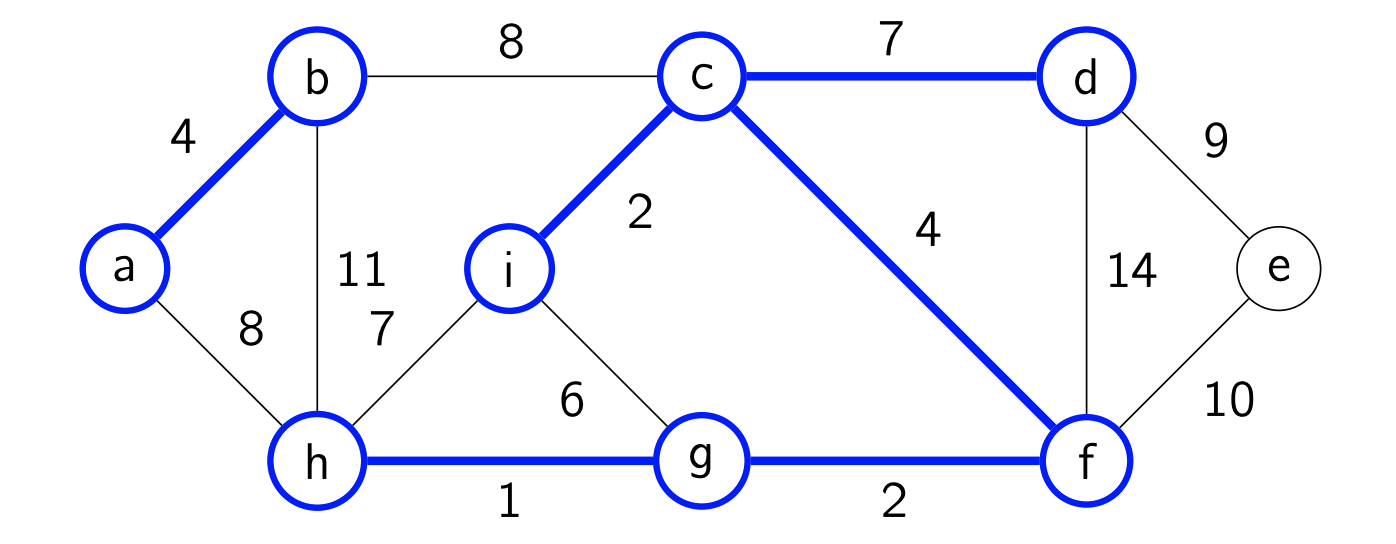
\includegraphics[scale=0.8]{kruskal6.png}
\caption{}
\label{fig:kruskal6}
\end{figure}

The next edge in the sorted order is $(h, i)$, but $h$ and $i$ are contained in the same set so we ignore it. The next edge is a tie between edges $(a, h)$ and $(b, c)$. Let’s say the algorithm picks $(a, h)$. We union the sets containing a and h and add edge $(a, h)$ to $A$ as shown in Figure \ref{fig:kruskal7}.


\begin{figure}[h!]
\centering
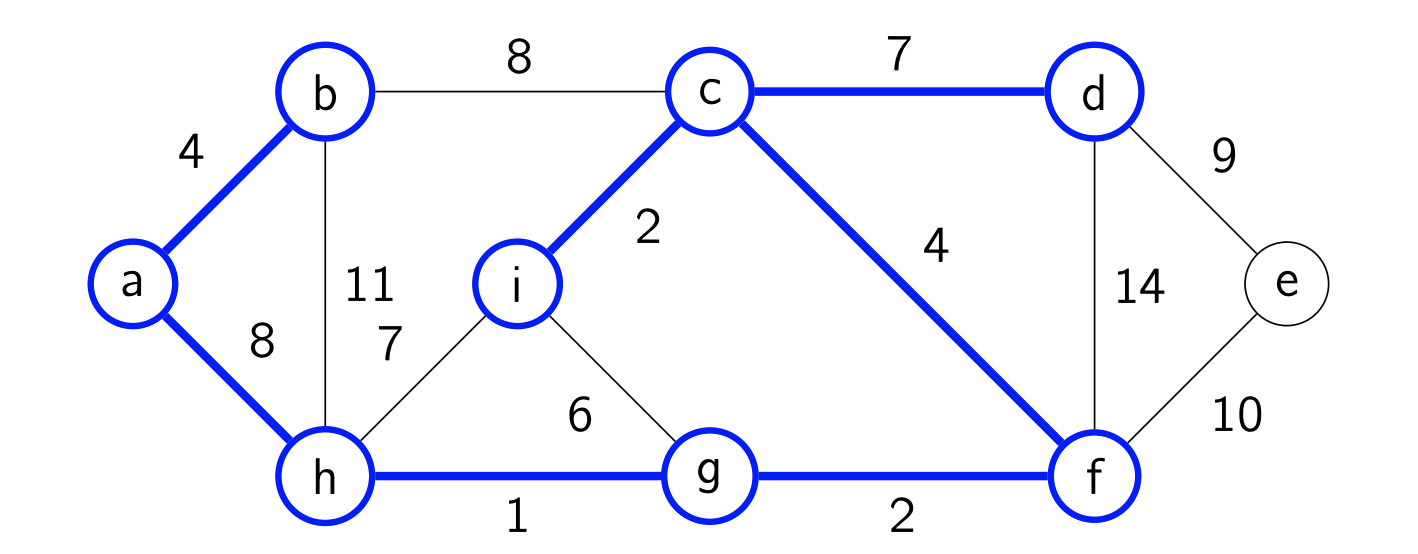
\includegraphics[scale=0.8]{kruskal7.png}
\caption{}
\label{fig:kruskal7}
\end{figure}

The next edge in the sorted order which has both vertices in different sets is $(d, e)$. We union the sets containing $ d$ and $e$ and add edge $(d, e)$ to $A$ as shown in Figure \ref{fig:kruskal8}. At this point all nodes are contained in the same set, so no further edges are added to A.


\begin{figure}[h!]
\centering
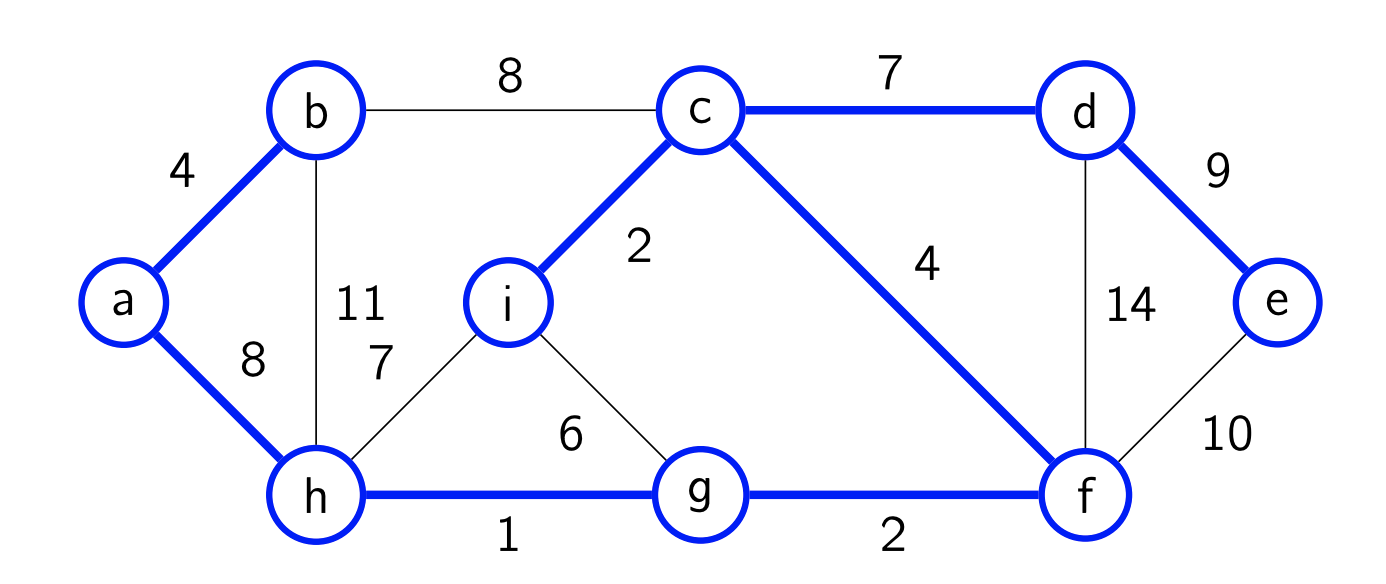
\includegraphics[scale=0.8]{kruskal8.png}
\caption{}
\label{fig:kruskal8}
\end{figure}


\section{The Latest and Greatest Algorithms}
 
While the greedy algorithms mentioned above are reasonably efficient ways to compute a minimum spanning tree of a graph, recent research has yielded more efficient algorithms. In 1995, Karger, Klein, and Tarjan discovered a randomized linear time $(O(E + V ))$ algorithm based on Borůvka's algorithm and the reverse-delete algorithm. In 2000, Chazelle discovered the current fastest determistic algorithm which runs in time $O(E \alpha(V ))$ using soft heaps where $\alpha$ is the inverse Ackermann function.






















\end{document}
